\documentclass[conference]{IEEEtran}
\IEEEoverridecommandlockouts
% The preceding line is only needed to identify funding in the first footnote. If that is unneeded, please comment it out.
\usepackage{cite}
\usepackage{amsmath,amssymb,amsfonts}
\usepackage{algorithmic}
\usepackage{graphicx}
\graphicspath{ {images/} }
\usepackage{textcomp}
\usepackage{xcolor}
\usepackage{caption}
\def\BibTeX{{\rm B\kern-.05em{\sc i\kern-.025em b}\kern-.08em
    T\kern-.1667em\lower.7ex\hbox{E}\kern-.125emX}}
\begin{document}

\title{Recurrent Neural Networks for object detection}

\author{\IEEEauthorblockN{1\textsuperscript{st} Bin Qasim Ahmad}
\IEEEauthorblockA{\textit{Technical University of Munich} \\
\textit{Department of Informatics}\\
Munich, Germany \\
ahmad.qasim@tum.de }
\and
\IEEEauthorblockN{2\textsuperscript{nd} Pettirsch Arnd}
\IEEEauthorblockA{\textit{Technical University of Munich)} \\
\textit{Department of Informatics}\\
Munich, Germany \\
a.pettirsch@outlook.de}
}

\maketitle

\begin{abstract}
ToDo
\end{abstract}

\begin{IEEEkeywords}
TBD.
\end{IEEEkeywords}

\section{Introduction}

\subsection{Image and Video Object Detection in general}
\begin{itemize}
	\item Image object detection history.
	\begin{itemize}
		\item Bayesian methods before deep learning
		\item ImageNet challenge and VID [15]
		\item Deep Learning and AlexNet [16]
	\end{itemize}
	\item Single stage and 2-stage image object detectors.
	\begin{itemize}
		\item A two-stage pipeline firstly generates region proposals, which are then classified and refined. [17]
		\item A single-stage method is often more efficient but less accurate. Directly regress on bounding boxes and classes. [18], [19]
	\end{itemize}
	\item Why is video object detection harder?
	\begin{itemize}
		\item Large size
		\item Motion blur
		\item Quality of the dataset
		\item Partial occlusion
		\item Unconventional Poses
	\end{itemize}
\end{itemize}

\subsection{Recurrent Neural Networks in general}
ToDo


\section{Feature-based Video Object Detection}

\subsection{Definition}
ToDo

\subsection{Recurrent Multi-fram Single Shot Detector for Video Object Detection}
ToDo

\subsection{Mobile Video Object Detection with Temporally Aware Feature Maps}
ToDo

\subsection{Feature Selective Small Object Detection via Knowledge-based recurrent attentive neural networks}
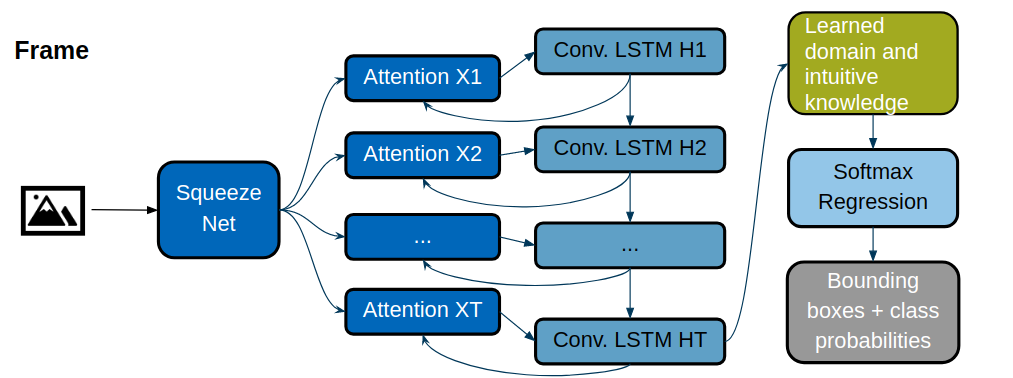
\includegraphics[width=\columnwidth]{KB-RANN-architecture}
\begin{itemize}
	\item Compute feature maps using a modified SqueezeNet architecture.
	\item Propagate the features through a Recurrent Attentive Neural Network, comprised of:
	\begin{itemize}
		\item Attention Mechanism to detect key areas within the feature maps.
		\item Convolutional LSTM for temporal feature propagation.	
	\end{itemize}
	\item Reverse gaussian feature maps are combined with the maps obtained from Conv. LSTM.
	\begin{itemize}
		\item These feature maps are based on learnable mean and covariance terms.
		\item This prior knowledge is derived from the assumption that traffic signs are always located at the bias of the center.

	\end{itemize}
\end{itemize}

\subsection{Looking fast and slow: memory-guided mobile video object detection}
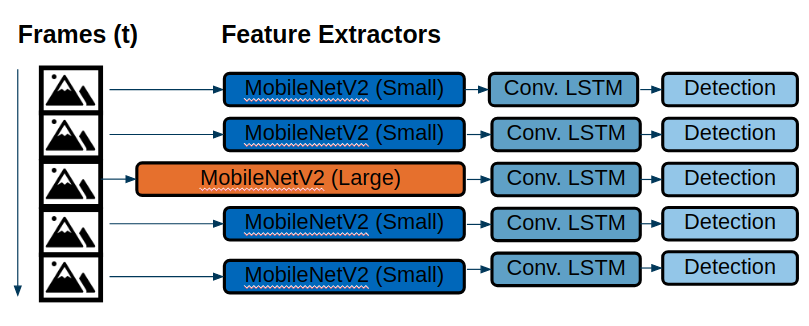
\includegraphics[width=\columnwidth]{looking-fast-and-slow-architecture}
\begin{itemize}
	\item Run multiple feature extractors sequentially or concurrently to obtain feature maps.
	\begin{itemize}
		\item 	The idea is to use small and large feature extractors to optimize performance.
	\end{itemize}
	\item Aggregate and refine these feature maps using convolutional LSTM based memory network.
	\begin{itemize}
		\item To improve speed of LSTM network, add skip connections and LSTM state groups.
	\end{itemize}
	\item Apply SSD-style detection on refined features to obtain classification and bounding boxes.
	\item Use a reinforcement learning based policy for selection of which feature extractor to run.
	\item Large and small frame extractors can run in parallel using asynchronous mode.
\end{itemize}

\subsection{Detect to Track and track to detect}
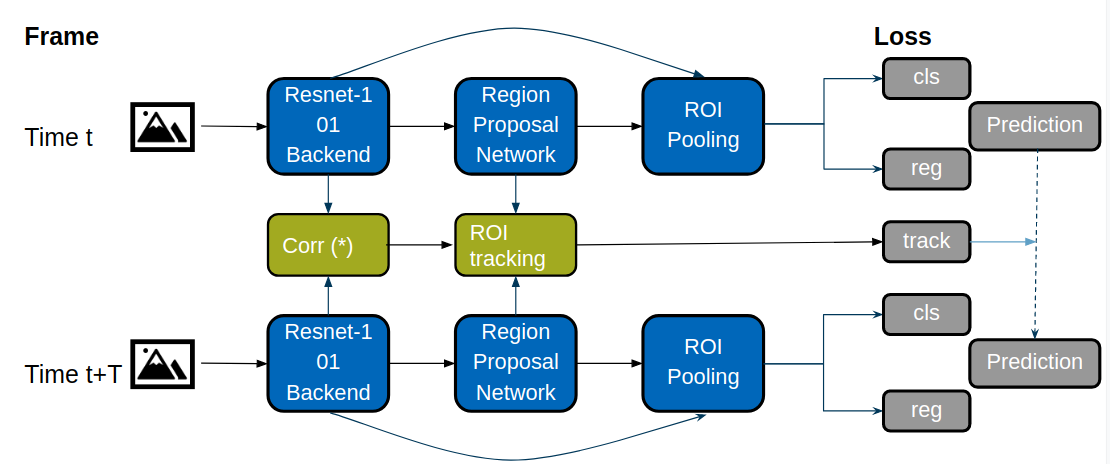
\includegraphics[width=\columnwidth]{D&T-architecture}
\begin{itemize}
	\item Compute Convolutional feature maps using a Resnet-101 architecture.
	\item Use a RPN (region proposal network) to find candidate regions in the frame.
	\item ROI Pooling layer, to classify boxes and refine their coordinates (regression).
	\item Find correlation features between two frames’ feature maps and do ROI tracking.
	\item Due to memory constraints, use tracklets, which are class-based optimal paths in video.

\end{itemize}

\section{Box-Level-based Video Object Detection}

\subsection{Definition}
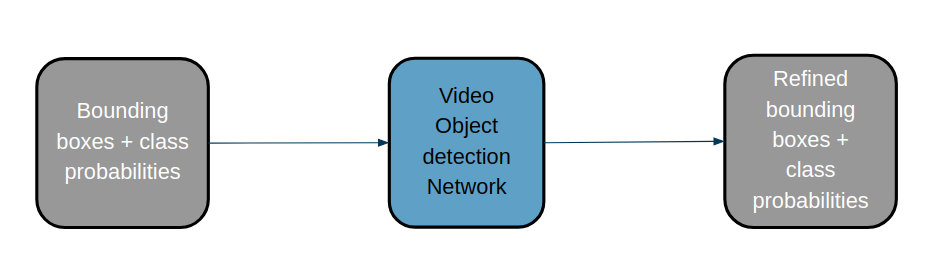
\includegraphics[width=\columnwidth]{box-level-basic}
Bounding Boxes and Class probabilities are fed into the network and are refined temporally and/or spatially.

\subsection{Object Detection from Video Tubelets with Convolutional Neural Networks}
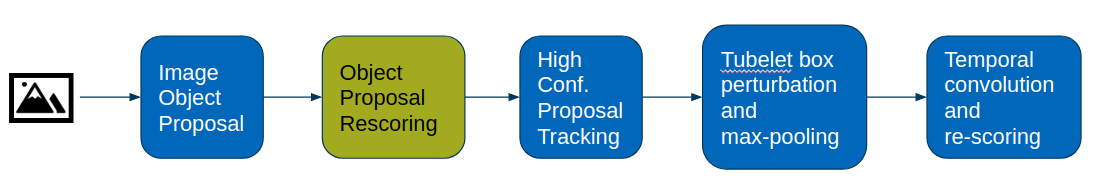
\includegraphics[width=\columnwidth]{video-tubelets-architecture}
\begin{itemize}
	\item Use selective search algorithm to generate around 2000 object proposals on each frame.
	\item Use GoogleNet for feature extraction and then 30 SVMs for 30 VID classes to generate object proposal scores for each object proposal.
	\item Track high confidence targets bi-directionally.
	\item Two kinds of Perturbations:
	\begin{itemize}
		\item The first method is to generate new boxes around each tubelet box on each frame by randomly perturbing the boundaries of the tubelet box.
		\item The second perturbation method is to replace each tubelet box with original object detections that have overlaps with the tubelet box beyond a threshold.	
	\end{itemize}
	\item Train a class-specific TCN using the tubelet features as input. The inputs are time series including detection scores, tracking scores and anchor offsets. The output values are probabilities whether each tubelet box contains objects of the class
\end{itemize}

\subsection{Optimizing Video Object Detection via Scale-Time Lattice}
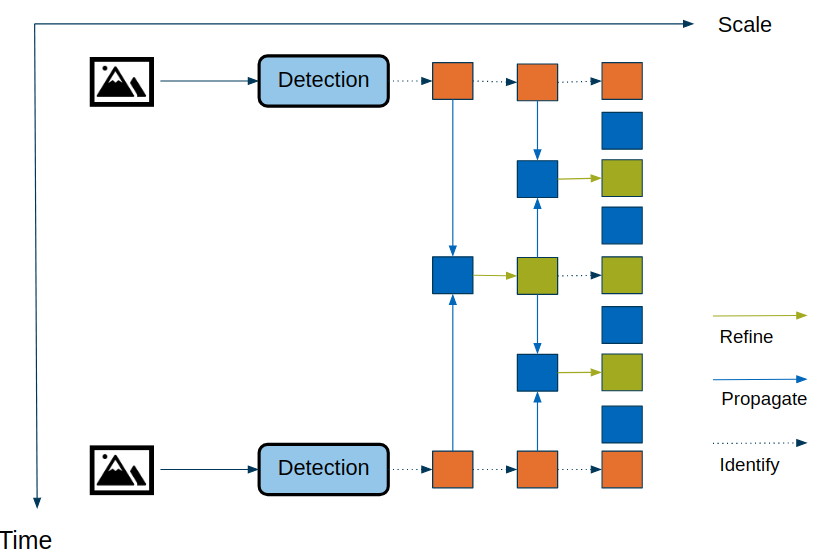
\includegraphics[width=\columnwidth]{scale-time-lattice}
\begin{itemize}
	\item Apply object detection on keyframes extracted adaptively.
	\begin{itemize}
		\item The extraction policy is based on number of objects and amount of movement in frames.
		\item If higher number/movement of objects in frames then higher extraction rate.
	\end{itemize}
	\item Propagation and refinement unit, propagates the frames temporally and refines spatially.
	\item For temporal propagation, use a small network such as resnet-18 to extract box features and a regressor to predict object movement from t to t + T.
	\item For spatial refinement, use a regressor to refine the bounding boxes over increasing scale.

\end{itemize}

\subsection{Context Matters: Refining Object Detection in Video with Recurrent Neural Networks}
ToDo

\subsection{Spatially Supervised Recurrent Convolutional Neural Networks for Visual Object Tracking}
ToDo


\section{Flow-based Object Detection}

\subsection{Definition}
Todo

\subsection{Deep Feature Flow for Video Recognition}
Todo

\section{Comparison of different approaches}

\subsection{General}
\captionof{table}{Results on KITTI Dataset} 
\begin{tabular}{ | p{2cm} | p{2em}| p{2em} | p{4em} | p{5em} | } 
 \hline
 Model & MAP & FPS & Machine & Architecture \\
 \hline
 Recurrent \cite{b1} & 86.0 & 50 & Nvidia TITAN X & Feature-Level \\
 \hline
 Feature Selective \cite{b6} & 81.3 & 30.8 & Nvidia TITAN X & Feature-Level \\
 \hline
\end{tabular}

\captionof{table}{Results on ImageNet Dataset} 
\begin{tabular}{ | p{2cm} | p{2em}| p{2em} | p{4em} | p{5em} | } 
 \hline
 Model & MAP & FPS & Machine & Architecture \\
 \hline
 DT \cite{b8} & 82.0 & 7 & Nvidia TITAN X & Feature-Level \\
 \hline
 DT \cite{b8} & 78.5 & 55 & Nvidia TITAN X & Feature-Level \\
 \hline
 Scale-Time Lattice \cite{b10} & 79.6 & 20 & Nvidia TITAN X & Box-Level \\
 \hline
 Scale-Time Lattice \cite{b10} & 79 & 62 & Nvidia TITAN X & Box-Level \\
 \hline
 DeepFeature Flow \cite{b3} & 73.9 & 3 & - & Flow-Based \\
 \hline
 DeepFeature Flow \cite{b3} & 73.1 & 20.5 & - & Flow-Based \\
 \hline
 Looking Fast and Slow \cite{b7} & 60.7 & 48.8 & Pixel Phone & Feature-Level \\
 \hline
 Object Detection with Temporally-Aware \cite{b2} & 54.4 & 15 & Pixel Phone & Feature-Level \\
 \hline
\end{tabular}

\captionof{table}{Results on COCO Dataset} 
\begin{tabular}{ | p{2cm} | p{2em}| p{2em} | p{4em} | p{5em} | } 
 \hline
 Model & MAP & FPS & Machine & Architecture \\
 \hline
 Feature Selective \cite{b6} & 57.8 & 37.5 & Nvidia TITAN X & Feature-Level \\
 \hline
\end{tabular}

\captionof{table}{Results on YT Dataset} 
\begin{tabular}{ | p{2cm} | p{2em}| p{2em} | p{4em} | p{5em} | } 
 \hline
 Model & MAP & FPS & Machine & Architecture \\
 \hline
 Context Matters \cite{b4} & 68.73 & - & - & Box-Level \\
 \hline
\end{tabular}

\captionof{table}{Results on OTB Challenge Dataset} 
\begin{tabular}{ | p{2cm} | p{3em}| p{2em} | p{4em} | p{4em} | } 
 \hline
 Model & Success Rate & IoU & FPS & Machine \\
 \hline
 Spatially Supervised \cite{b5} & 0.564 & 0.455 & 20/60 & Nvidia TITAN X \\
 \hline
\end{tabular}
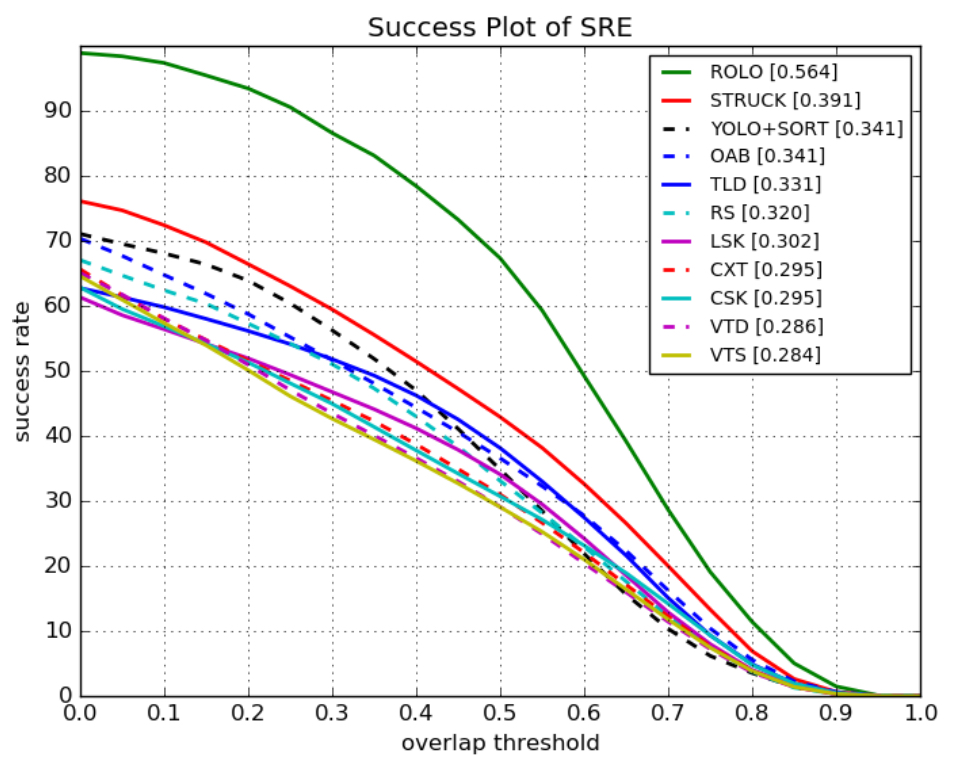
\includegraphics[width=\columnwidth]{otb-challenge-results}

\subsection{Conclusion Perfomance}
Todo

\subsection{Conclusion Prediction Quality}
Todo


\section{Outro}

\subsection{Conclusion}
Todo

\subsection{Further work}
Todo


\section*{Acknowledgment}
Todo

\section*{References}

Please number citations consecutively within brackets \cite{b1}. The 
sentence punctuation follows the bracket \cite{b2}. Refer simply to the reference 
number, as in \cite{b3}---do not use ``Ref. \cite{b3}'' or ``reference \cite{b3}'' except at 
the beginning of a sentence: ``Reference \cite{b3} was the first $\ldots$''

Number footnotes separately in superscripts. Place the actual footnote at 
the bottom of the column in which it was cited. Do not put footnotes in the 
abstract or reference list. Use letters for table footnotes.

Unless there are six authors or more give all authors' names; do not use 
``et al.''. Papers that have not been published, even if they have been 
submitted for publication, should be cited as ``unpublished'' \cite{b4}. Papers 
that have been accepted for publication should be cited as ``in press'' \cite{b5}. 
Capitalize only the first word in a paper title, except for proper nouns and 
element symbols.

For papers published in translation journals, please give the English 
citation first, followed by the original foreign-language citation \cite{b6}.

\begin{thebibliography}{00}
\bibitem{b1} Alexander Broad, Michael Jones, Teng-Yok Lee. Recurrent Multi-frame Single Shot Detector for Video Object Detection. 2018.
\bibitem{b2} Mason Liu, Menglong Zhu. Mobile Video Object Detection with Temporally-Aware Feature Maps. 2018.
\bibitem{b3} Xizhou Zhu, Yuwen Xiong, Jifeng Dai, Lu Yuan, Yichen Wei. Deep Feature Flow for Video Recognition. 2017.
\bibitem{b4} Subarna Tripathi, Zachary C. Lipton, Serge Belongie, Truong Nguyen. Context Matters: Refining Object Detection in Video with Recurrent Neural Networks.
\bibitem{b5} Guanghan Ning, Zhi Zhang, Chen Huang, Zhihai He, Xiaobo Ren, Haohong Wang. Spatially Supervised Recurrent Convolutional Neural Networks for Visual Object Tracking. 2016.
\bibitem{b6} Kai Yi, Zhiqiang Jian, Shitao Chen, Nanning Zheng. Feature Selective Small Object Detection via Knowledge-based Recurrent Attentive Neural Network. 2019.
\bibitem{b7} Mason Liu, Menglong Zhu, Marie White, Yinxiao Li, Dmitry Kalenichenko. Looking Fast and Slow: Memory-Guided Mobile Video Object Detection. 2019.
\bibitem{b8} Christoph Feichtenhofer, Axel Pinz, Andrew Zisserman. Detect to Track and Track to Detect. 2017.
\bibitem{b9} Kai Kang, Wanli Ouyang, Hongsheng Li, Xiaogang Wang. Object Detection from Video Tubelets with Convolutional Neural Networks. 2016.
\bibitem{b10} Kai Chen, Jiaqi Wang, Shuo Yang, Xingcheng Zhang, Yuanjun Xiong, Chen Change Loy, Dahua Lin. Optimizing Video Object Detection via a Scale-Time Lattice. 2018.
\bibitem{b11} Ian Goodfellow, Yoshua Bengio, Aaron Courville. Deep Learning (Adaptive Computation and Machine Learning). 2017.
\bibitem{b12} Alexander Broad, Michael Jones, Teng-Yok Lee. Supplementary Material for Recurrent Multi-frame Single Shot Detector for Video Object Detection. 2018.
\bibitem{b13} Jia Deng, Wei Dong, Richard Socher, Li-Jia Li, Kai Li and Li Fei-Fei. ImageNet: A Large-Scale Hierarchical Image Database. 
\bibitem{b14} Alex Krizhevsky, Ilya Sutskever, Geoffrey E. Hinton. ImageNet Classification with Deep Convolutional Neural Networks. 2012.
\bibitem{b15} Shaoqing Ren, Kaiming He, Ross Girshick, Jian Sun. Faster R-CNN: Towards Real-Time Object Detection with Region Proposal Networks. 2016. 
\bibitem{b16} Joseph Redmon, Ali Farhadi. YOLOv3: An Incremental Improvement.
\bibitem{b17} Wei Liu, Dragomir Anguelov, Dumitru Erhan, Christian Szegedy, Scott Reed, Cheng-Yang Fu, Alexander C. Berg. SSD: Single Shot MultiBox Detector. 2016.
\end{thebibliography}
\vspace{12pt}

\end{document}
